\chapter{Ocenjevanje modelov}
\label{ch:ocnjevanje-modelov}

Pogledali smo si logistični model -- lisice, ptice, kralje. Shema glasovanja je izgledala smiselna. Pred tem pa smo videli napovedi modela. Tudi te so bile točne. Kako pa bi lahko izračunali točnost modela?

Morda lahko izračunamo zgolj razmerje pravilno napovedanih pravljic? Taka mera se imenuje \textit{napovedna točnost (classification accuracy)}. Na primer, če smo pravilno napovedali 40 pravljic izmed 44, bo naša napovedna točnost 40/44 oziroma 91\%.

\begin{figure}[h]
    \centering
    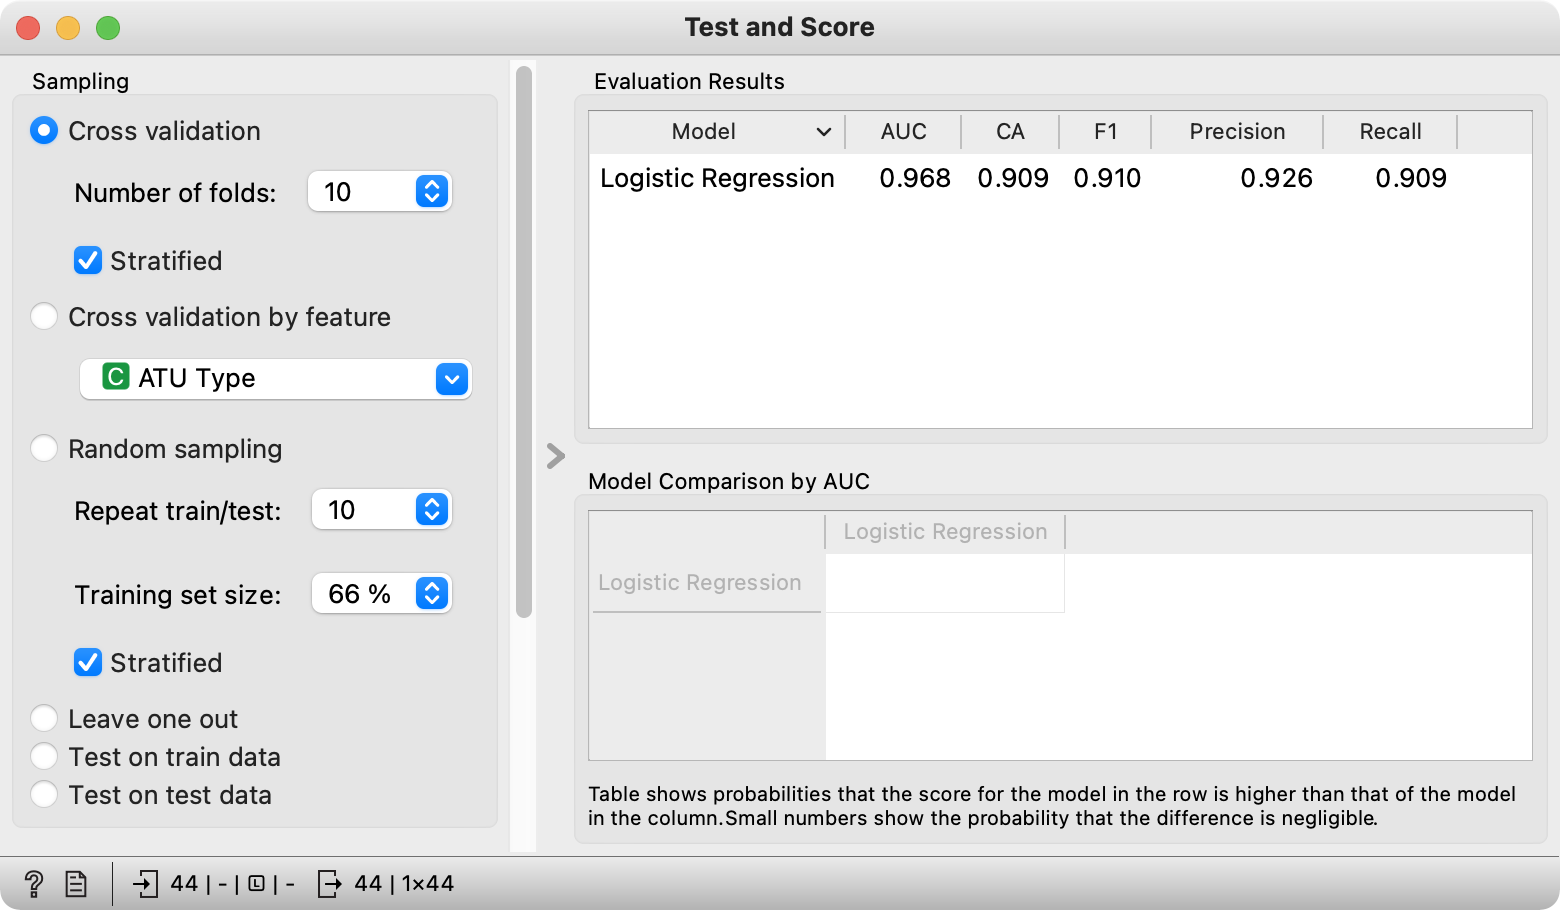
\includegraphics[width=0.95\linewidth]{test-and-score.png}%
    \caption{ }
    \label{fig:008-test-and-score}
\end{figure}
  
\textit{AUC} je ena izmed boljših mer točnosti. Na kratko, bližje ko je mera vrednosti 1, boljša je točnost modela.

Gradnik za računanje točnosti modela se imenuje \textit{Test \& Score}. Potrebuje dva vhoda: podatke za testiranje modela in napovedni postopek.

\begin{figure}[h]
    \centering
    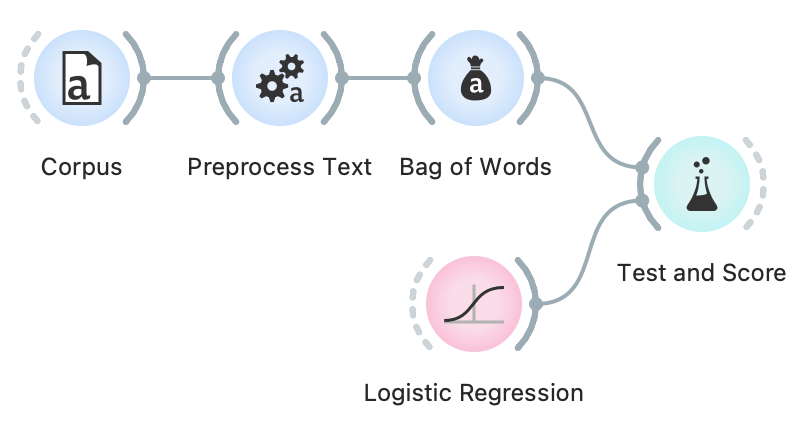
\includegraphics[width=0.6\linewidth]{ocenjevanje-workflow.png}%
    \caption{``Ni ravno smiselno, da vprašamo model, ali je Zlatolaska živalska pravljica, če smo modelu že pred tem povedali, da je magična.''

    Kaj nismo tega storili zgoraj v gradniku Predictions? Prav zares in zato so bile napovedi tako dobre. Modelov se nikoli ne sme preverjati na podatkih, ki smo jih jim dali za učenje.}
    \label{fig:008-ocnjevanje-workflow}
\end{figure}
  
Tokrat logistična regresija ne potrebuje vhodnih podatkov. Namesto tega bo gradnik podal postopek za gradnjo modela. Nato bo Test \& Score v več ponovitvah uporabil postopek na različnih podmnožicah podatkov. V vsaki ponovitvi bo naučil model na izbrani podmnožici in uporabil podatke izven množice za testiranje. Ni ravno smiselno, da vprašamo model, ali je Zlatolaska živalska pravljica, če smo modelu že pred tem povedali, da je magična.